% =============================================================================
%  T1 / P1 - Limiarizacao de imagens e video   |   VERSAO 2
%  Processamento de Imagens - UFMA
%
%  17 slides, dimensionados para 20 MINUTOS com 3 apresentadores
%  (~6 min cada). Compilar com XeLaTeX:
%      latexmk -xelatex apresentacao_v2.tex
% =============================================================================

\documentclass[aspectratio=169,12pt]{beamer}

% -----------------------------------------------------------------------------
%  >>> PREENCHA AQUI <<<
% -----------------------------------------------------------------------------
\newcommand{\alunoA}{Nome do Aluno A}
\newcommand{\alunoB}{Nome do Aluno B}
\newcommand{\alunoC}{Nome do Aluno C}
\newcommand{\professor}{Prof. Fulano de Tal}
% -----------------------------------------------------------------------------

\usetheme[progressbar=none, numbering=fraction, block=fill]{metropolis}

\usepackage{fontspec}
\setsansfont{Fira Sans}[Numbers=Lining]
\setmonofont{Fira Mono}[Scale=0.82]
\usepackage[brazil]{babel}
\usepackage{amsmath, amssymb}
\usepackage{booktabs}
\usepackage{array}
\usepackage{graphicx}

\graphicspath{{figuras/}{../resultados/graficos/}{../data/imagens/}}

\definecolor{ink}{HTML}{16262E}
\definecolor{cinza}{HTML}{5A6B73}
\definecolor{papel}{HTML}{FAFAF8}
\definecolor{marca}{HTML}{9A3B26}

\setbeamercolor{normal text}{fg=ink, bg=papel}
\setbeamercolor{alerted text}{fg=marca}
\setbeamercolor{frametitle}{bg=ink, fg=papel}
\setbeamercolor{title separator}{fg=marca}
\setbeamerfont{frametitle}{size=\large}

% legenda de figura: menor e em cinza
\newcommand{\leg}[1]{{\small\textcolor{cinza}{#1}}}

\setbeamertemplate{itemize items}[circle]
\setlength{\parskip}{.35em}

\title{Limiarização de imagens e vídeo}
\subtitle{Otsu, Multi-Otsu e limiarização adaptativa}
\author{\alunoA \quad \alunoB \quad \alunoC}
\institute{Processamento de Imagens \\ Universidade Federal do Maranhão \\ \professor}
\date{Trabalho T1}

\begin{document}

\maketitle

% =============================================================================
\begin{frame}{Limiarização}

  Segmentar comparando cada pixel com um valor de corte $T$:

  \vspace{-.7em}
  \[
    g(x,y) = 1 \;\text{ se } I(x,y) > T \;\text{ (objeto)},
    \qquad
    g(x,y) = 0 \;\text{ caso contrário}
  \]

  \vspace{-.5em}
  Uma comparação por pixel, sem treinamento. A dificuldade está em escolher $T$.

  \vspace{.7em}
  As três formas de escolher que estudamos:

  \begin{itemize}
    \item \textbf{Otsu}: um único $T$ para a imagem toda, tirado do histograma.
    \item \textbf{Multi-Otsu}: $M-1$ limiares, para cenas com mais de duas
      populações de cinza.
    \item \textbf{Adaptativa}: um $T$ diferente para cada pixel.
  \end{itemize}

\end{frame}

% =============================================================================
\begin{frame}{Modelo de formação da imagem}

  \begin{center}
    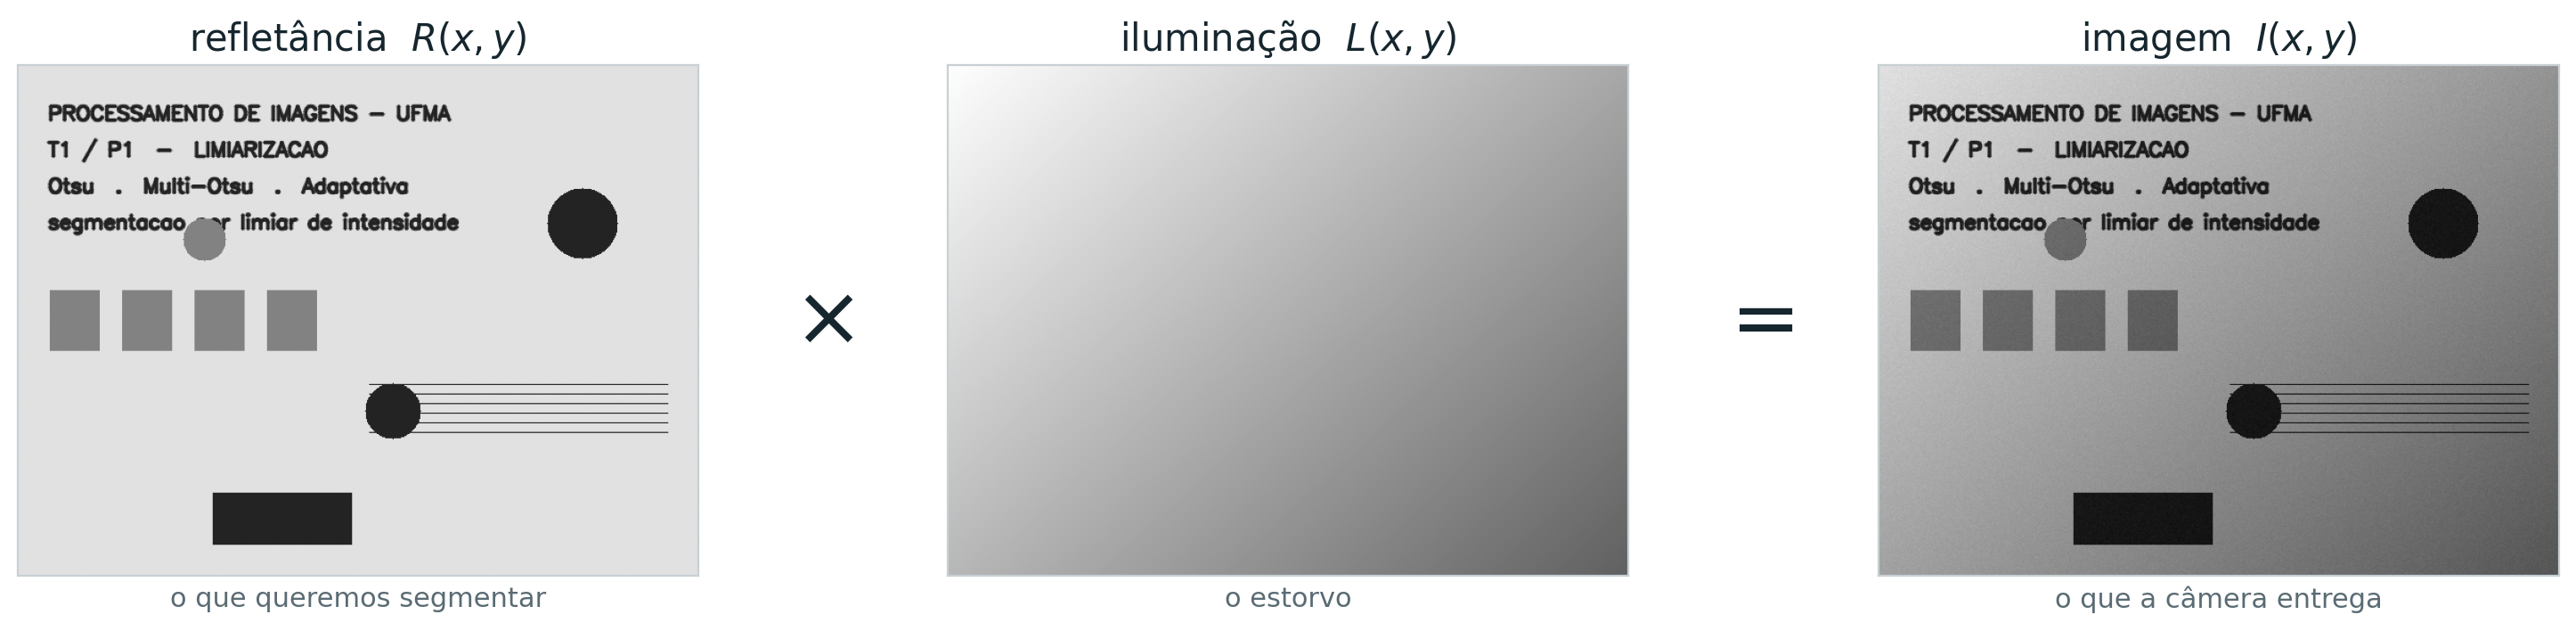
\includegraphics[width=\textwidth]{modelo_formacao}
  \end{center}

  \[
    I(x,y) = R(x,y)\cdot L(x,y) + n(x,y)
  \]

  \vspace{-.4em}
  Um limiar global só é válido se a iluminação $L$ for aproximadamente constante
  na imagem. Se a luz varia dentro da cena, o fundo de uma região escura fica
  mais escuro que o objeto de uma região clara.

\end{frame}

% =============================================================================
\begin{frame}{Material e método}

  \begin{center}
    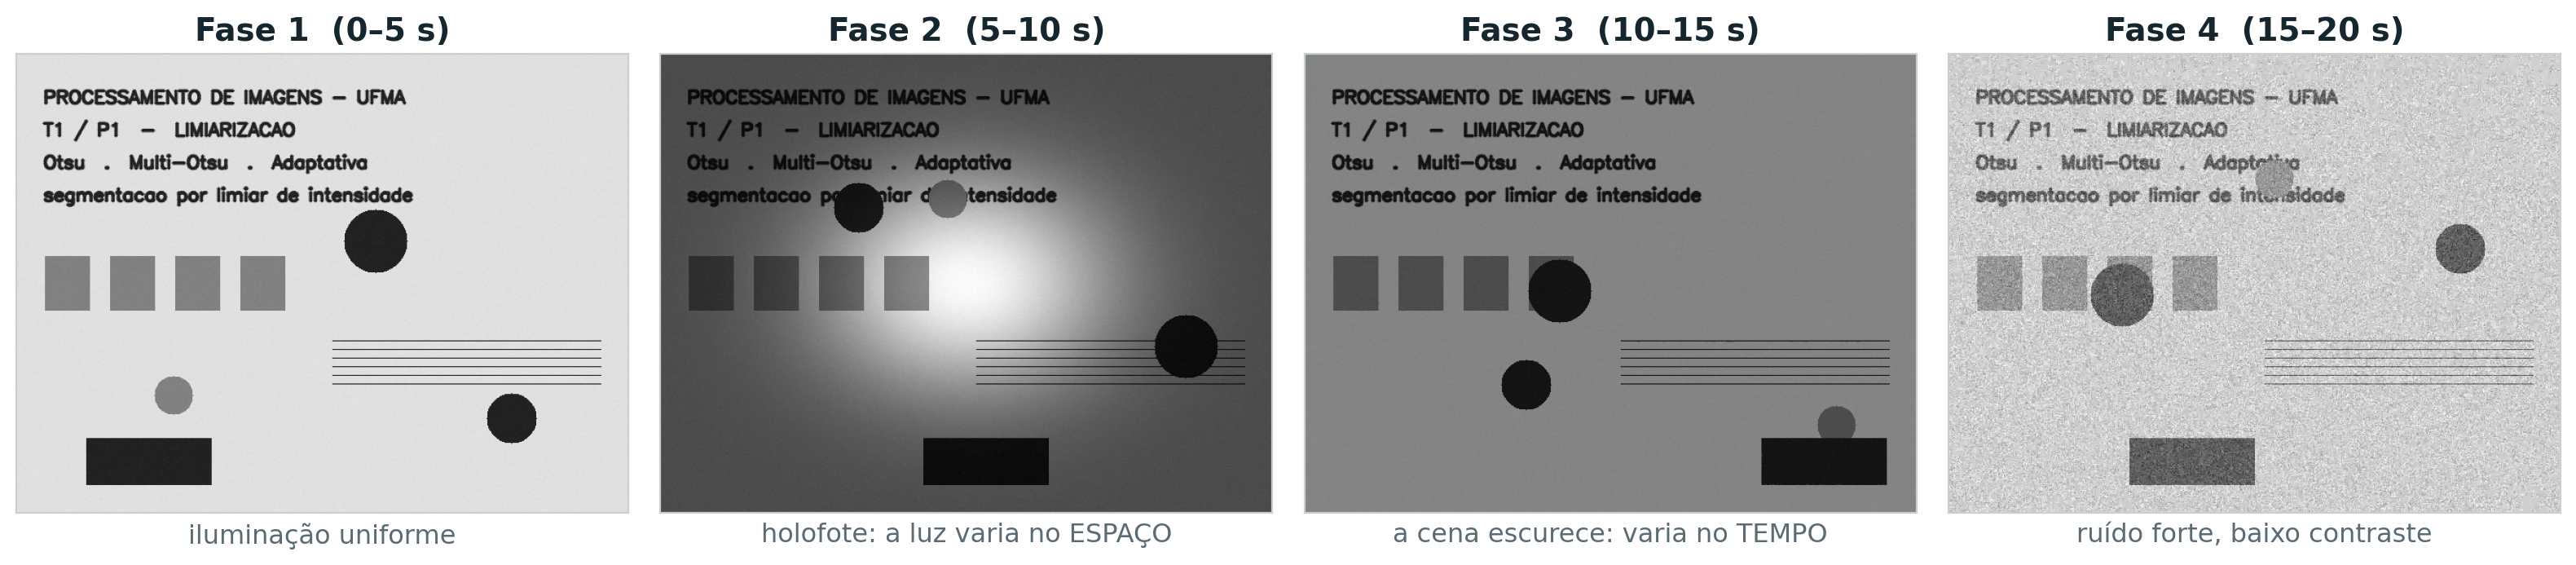
\includegraphics[width=\textwidth]{strip_fases}
  \end{center}

  \vspace{-.2em}
  Vídeo de 20~s (600 quadros, 640$\times$480) gerado com gabarito conhecido em
  cada quadro, dividido em quatro fases. Também foram usadas três imagens do
  acervo do scikit-image (\texttt{camera}, \texttt{coins}, \texttt{page}).

  \vspace{.3em}
  Métrica: $\mathrm{IoU} = VP/(VP+FP+FN)$. A acurácia não serve aqui, porque o
  objeto ocupa apenas 12\,\% da área.

\end{frame}

% =============================================================================
\section{Otsu}

% -----------------------------------------------------------------------------
\begin{frame}{Método de Otsu (1979)}

  O histograma normalizado $p(i)$ é tratado como distribuição de probabilidade.
  Um limiar $t$ separa duas classes, com pesos $\omega_k$ e médias $\mu_k$.

  \vspace{.3em}
  \begin{columns}[T,onlytextwidth]
    \column{.47\textwidth}
      Variância dentro das classes:
      \[ \sigma_W^2(t)=\omega_0\sigma_0^2+\omega_1\sigma_1^2 \]
    \column{.47\textwidth}
      Variância entre as classes:
      \[ \sigma_B^2(t)=\omega_0\,\omega_1\,(\mu_0-\mu_1)^2 \]
  \end{columns}

  \vspace{.5em}
  Vale a identidade $\sigma_T^2 = \sigma_W^2(t) + \sigma_B^2(t)$, e $\sigma_T^2$
  não depende de $t$. Logo maximizar $\sigma_B^2$ equivale a minimizar
  $\sigma_W^2$, e o critério é

  \[ t^{*} = \arg\max_t \;\sigma_B^2(t) \]

  \vspace{-.2em}
  Custo $O(N)$, uma passada pela imagem: 0,16~ms por quadro de 640$\times$480.

\end{frame}

% -----------------------------------------------------------------------------
\begin{frame}{Otsu: histograma e critério}

  \begin{center}
    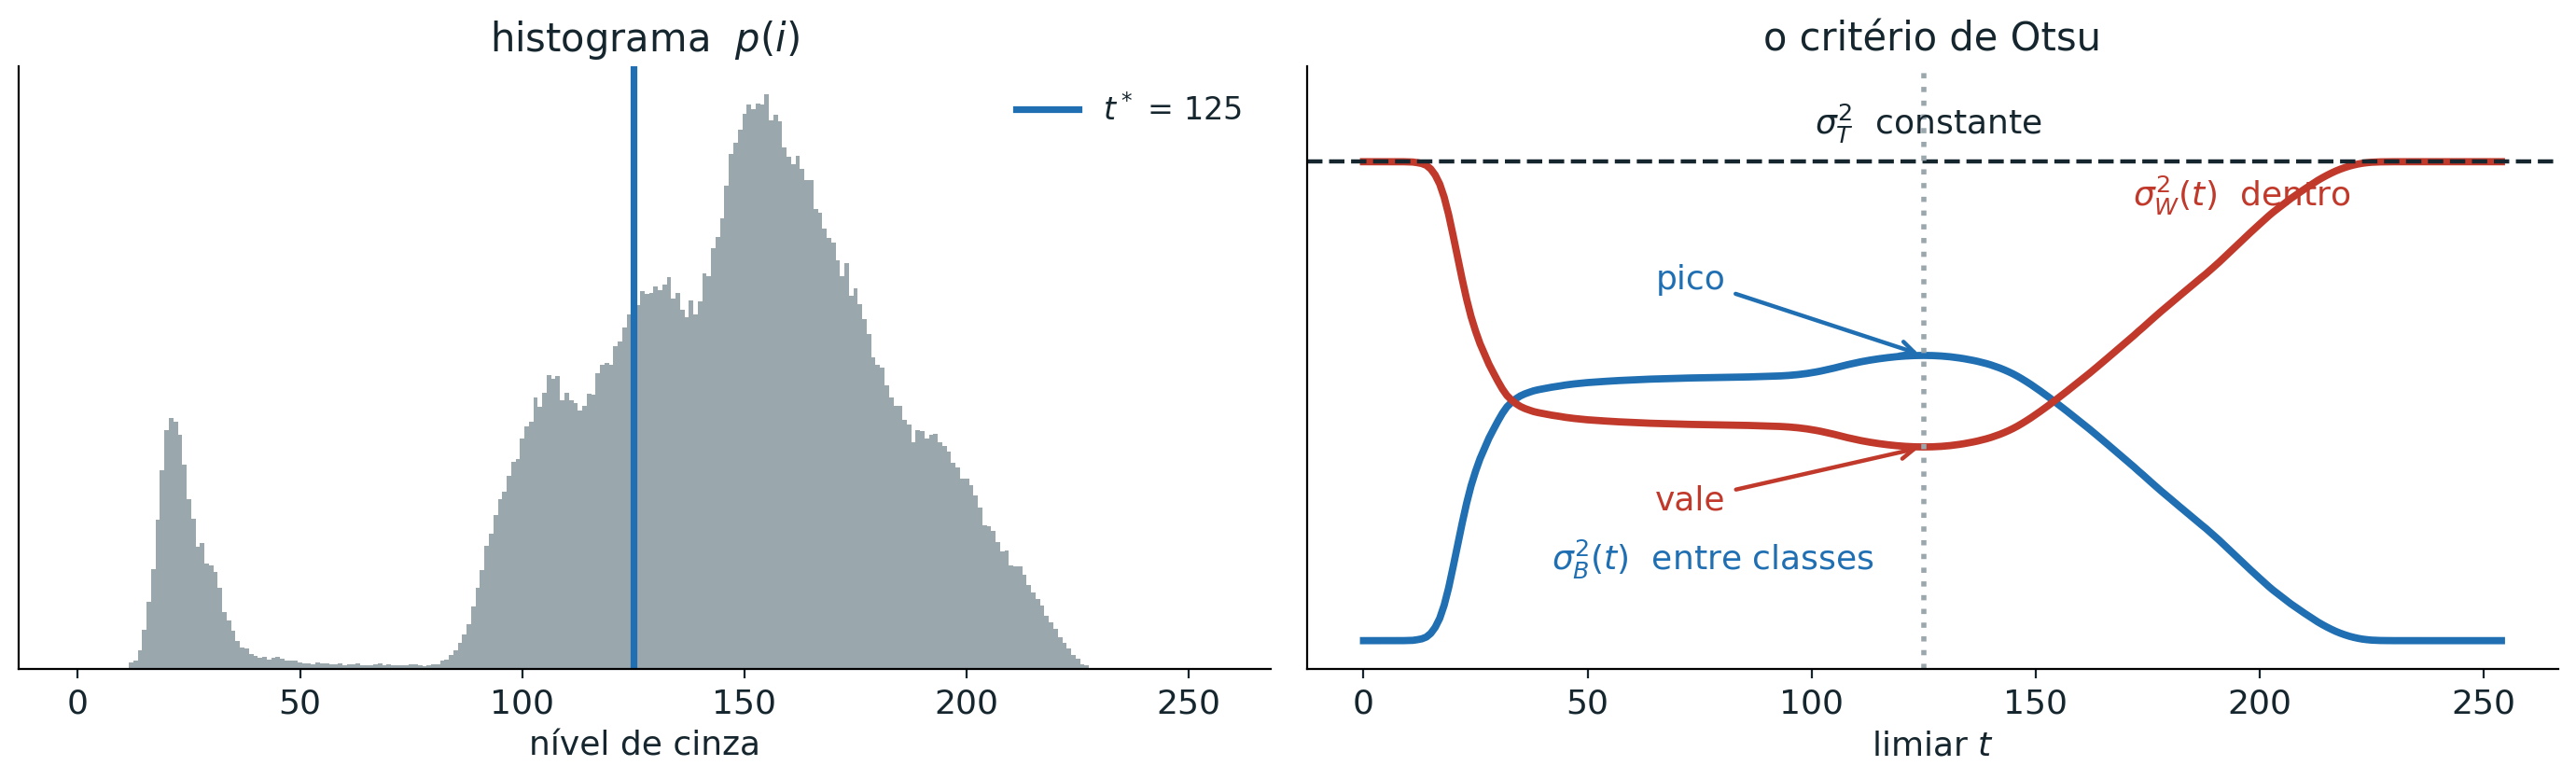
\includegraphics[width=\textwidth]{otsu_anatomia}
  \end{center}

  \leg{O pico da variância entre classes coincide com o vale da variância dentro
  das classes, e a soma das duas é constante. O limiar escolhido é o do pico.}

\end{frame}

% -----------------------------------------------------------------------------
\begin{frame}{Otsu no vídeo}

  \begin{columns}[T,onlytextwidth]
    \column{.46\textwidth}
      \textbf{Fase 3, a cena escurece}

      \medskip
      O limiar cai sozinho de 147 para 47 e o IoU permanece em 0,94.

      \medskip
      Otsu é invariante a mudanças globais de iluminação, porque recalcula o
      limiar a cada quadro.

    \column{.46\textwidth}
      \textbf{Fase 2, holofote}

      \medskip
      O IoU cai para 0,139.

      \medskip
      Com variação espacial da luz nenhum limiar único funciona. O método acha
      o melhor $T$, mas o melhor $T$ não resolve.
  \end{columns}

  \vspace{1.6em}
  O problema do limiar global não é iluminação variável em geral, e sim
  iluminação que varia \alert{dentro} da imagem.

\end{frame}

% =============================================================================
\section{Multi-Otsu}

% -----------------------------------------------------------------------------
\begin{frame}{Multi-Otsu}

  Muitas cenas têm mais de duas populações de cinza: documento com papel, tinta
  e sombra; radiografia com fundo, tecido e osso. Forçar duas classes funde duas
  populações distintas.

  \vspace{.4em}
  O critério é a extensão direta do de Otsu para $M$ classes e $M-1$ limiares:

  \[
    \sigma_B^2(t_1,\dots,t_{M-1}) = \sum_{k=0}^{M-1}\omega_k\,(\mu_k-\mu_T)^2
  \]

  \vspace{-.2em}
  A saída não é binária, e sim um mapa de rótulos (\texttt{np.digitize}).
  Para obter uma máscara binária é preciso decidir em qual limiar cortar, e essa
  decisão é do projetista.

\end{frame}

% -----------------------------------------------------------------------------
\begin{frame}{O custo da busca}

  \begin{columns}[c,onlytextwidth]
    \column{.44\textwidth}
      \footnotesize
      \begin{tabular}{@{}ccr@{}}
        \toprule
        $M$ & limiares & combinações \\
        \midrule
        2 & 1 & 255 \\
        3 & 2 & 32\,385 \\
        4 & 3 & 2\,731\,135 \\
        5 & 4 & 172\,061\,505 \\
        \bottomrule
      \end{tabular}

      \vspace{.8em}
      \normalsize
      A busca exaustiva testa $\binom{L-1}{M-1}$ combinações e se torna
      inviável a partir de $M=5$.

    \column{.52\textwidth}
      Solução em duas partes:

      \begin{itemize}
        \item tabelas de momentos (Liao, Chen \& Chung, 2001), com
          $H(u,v) = S(u,v)^2/P(u,v)$;
        \item programação dinâmica sobre essas tabelas,
          $D[m][v]=\max_{u<v}\bigl(D[m{-}1][u]+H(u{+}1,v)\bigr)$.
      \end{itemize}

      \vspace{.4em}
      O custo cai para $O(M L^2)$, cerca de 1,3~ms para $M=3$.
  \end{columns}

\end{frame}

% -----------------------------------------------------------------------------
\begin{frame}{Multi-Otsu: resultado}

  \begin{center}
    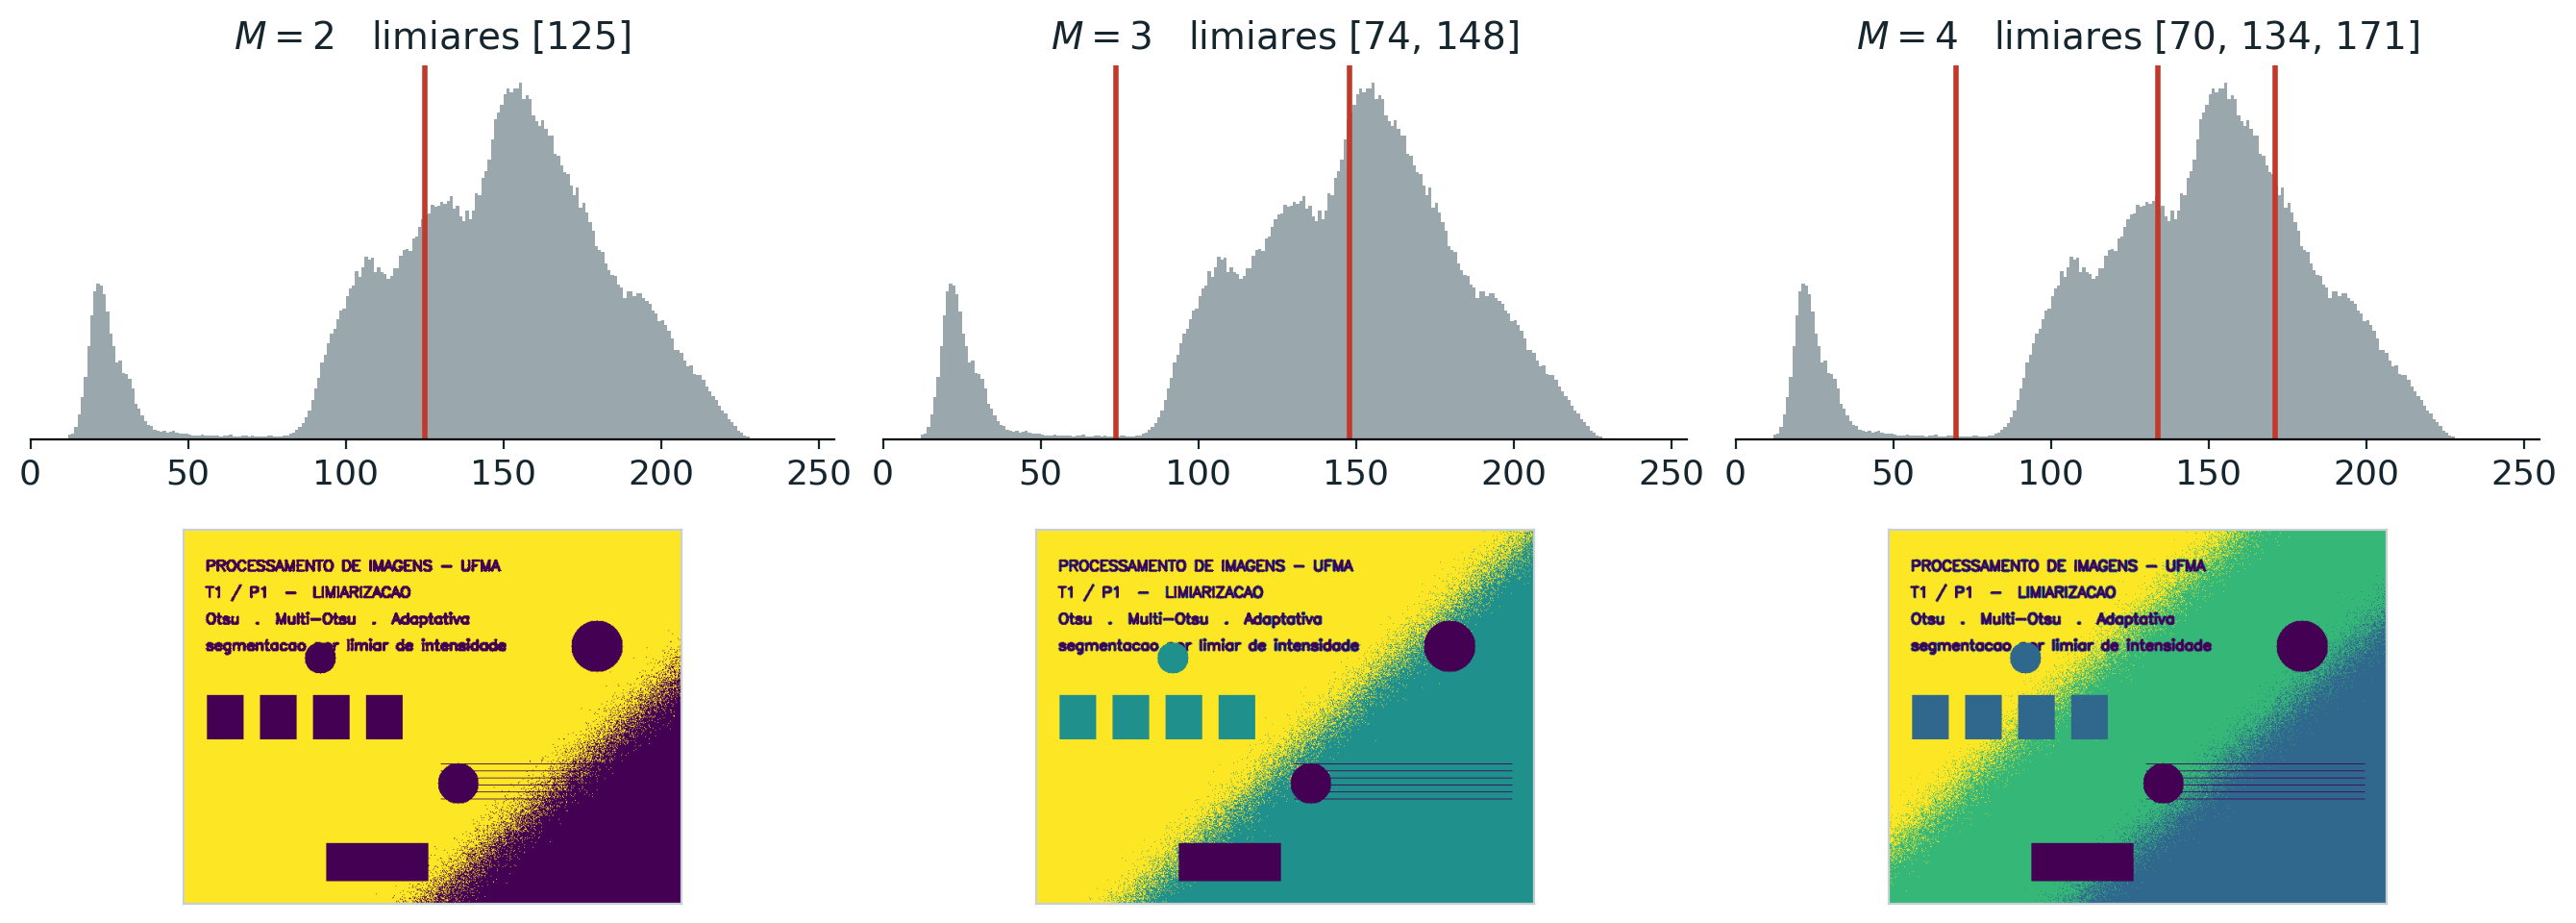
\includegraphics[width=.82\textwidth]{multiotsu_M_slide}
  \end{center}

  \vspace{-.3em}
  Aumentar $M$ sempre aumenta $\sigma_B^2$, então $M$ não pode ser escolhido
  maximizando o próprio critério: é um hiperparâmetro.

  \vspace{.3em}
  Com luz uniforme, cortar em $t_2$ dá IoU 0,966, o melhor entre os métodos
  globais. Sob o holofote $t_2$ cai para 0,138, enquanto $t_1$ mantém 0,731.

\end{frame}

% =============================================================================
\section{Limiarização adaptativa}

% -----------------------------------------------------------------------------
\begin{frame}{Limiarização adaptativa}

  \begin{center}
    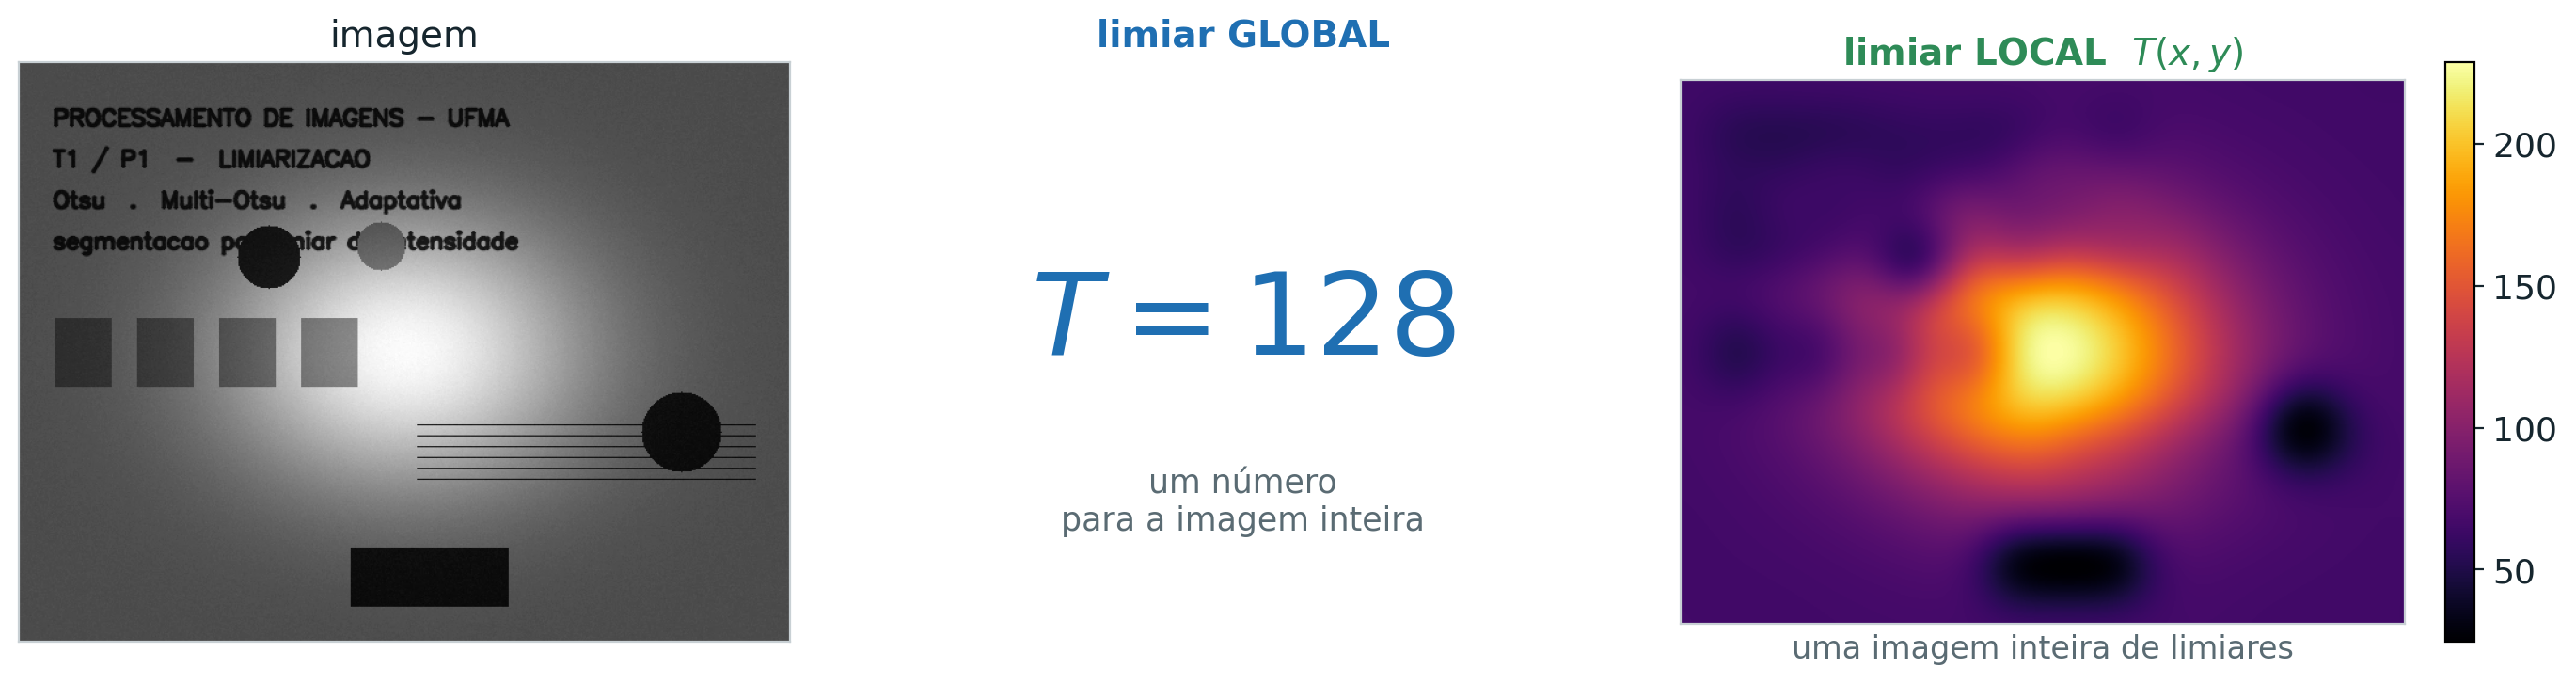
\includegraphics[width=.92\textwidth]{limiar_global_vs_local}
  \end{center}

  \vspace{-.2em}
  O limiar deixa de ser um número e passa a ser uma imagem, calculada a partir
  da vizinhança $b \times b$ de cada pixel:

  \[
    T(x,y) = m(x,y) - C
  \]

  \vspace{-.3em}
  \leg{$m$ é a média da vizinhança (\texttt{ADAPTIVE\_THRESH\_MEAN\_C}) ou a
  média ponderada por uma gaussiana (\texttt{ADAPTIVE\_THRESH\_GAUSSIAN\_C}).}

\end{frame}

% -----------------------------------------------------------------------------
\begin{frame}{Os dois parâmetros}

  \begin{center}
    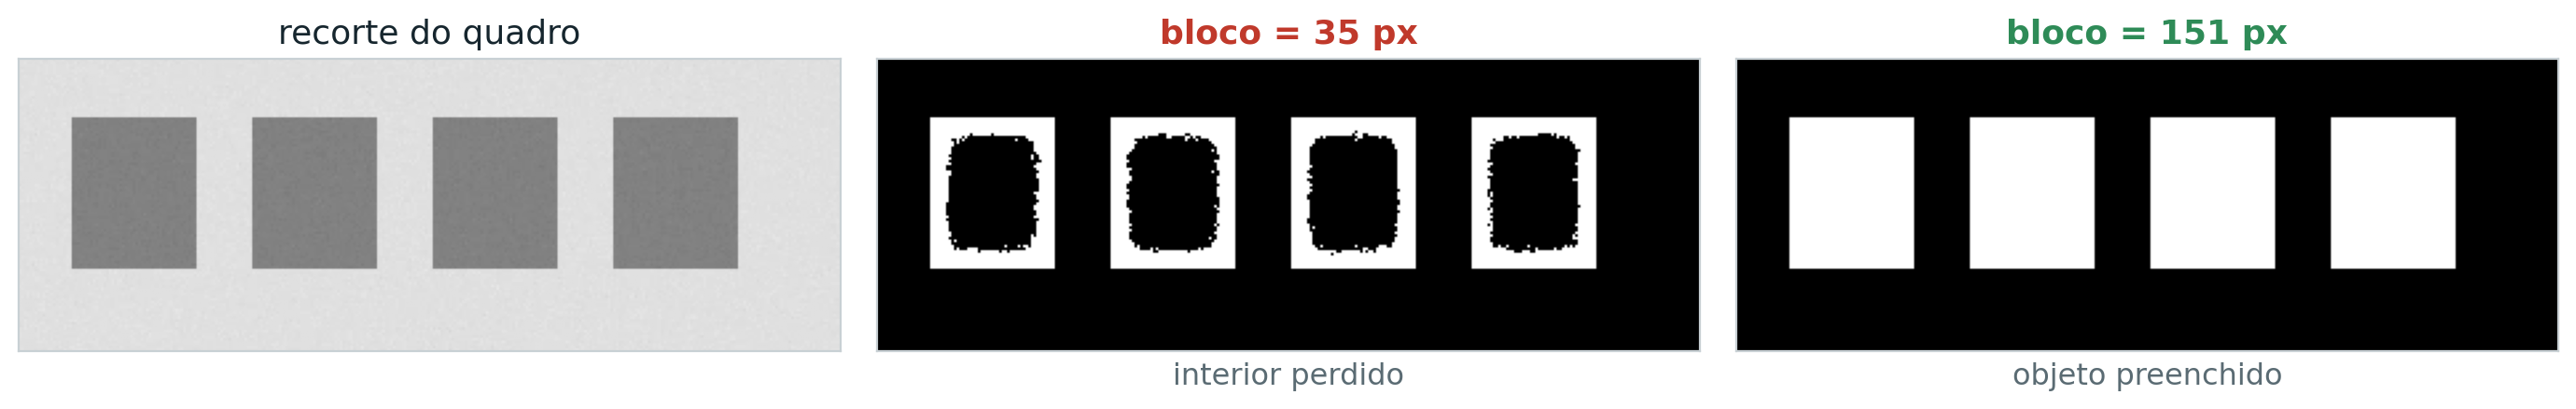
\includegraphics[width=.92\textwidth]{esvaziamento}
  \end{center}

  \vspace{-.2em}
  \begin{columns}[T,onlytextwidth]
    \column{.47\textwidth}
      \textbf{Bloco $b$.} No centro de um objeto grande a vizinhança inteira cai
      dentro do objeto, $m \approx I$, e só a borda sobrevive. O bloco precisa
      ser maior que o objeto e menor que a escala de variação da luz.

    \column{.47\textwidth}
      \textbf{Constante $C$.} Em região homogênea $I \approx m$, e sem $C$ o
      resultado seria ruído puro. $C$ cria uma margem: só é objeto o pixel ao
      menos $C$ níveis mais escuro que a vizinhança.
  \end{columns}

  \vspace{.6em}
  Com $b=35$ o IoU médio no vídeo foi 0,513; com $b=151$, 0,863.

\end{frame}

% -----------------------------------------------------------------------------
\begin{frame}{Custo}

  A média em janela $b\times b$ seria $O(N b^2)$. Com a imagem integral
  $II(x,y)=\sum_{x'\le x}\sum_{y'\le y} I(x',y')$, a soma de qualquer retângulo
  sai com quatro acessos e o custo cai para $O(N)$, independente do tamanho da
  janela.

  \vspace{.8em}
  \begin{center}
  \footnotesize
  \begin{tabular}{@{}lrr@{}}
    \toprule
    Método & ms/quadro & fps \\
    \midrule
    Otsu (OpenCV) & 0,16 & 6\,370 \\
    Multi-Otsu $M=3$ & 1,20 & 830 \\
    Adaptativa $b=35$ & 4,62 & 216 \\
    Adaptativa $b=151$ & 22,8 & 44 \\
    \bottomrule
  \end{tabular}
  \end{center}

  \vspace{.3em}
  \leg{Quadros de 640$\times$480. Todos rodam em tempo real a 30~fps.}

\end{frame}

% =============================================================================
\section{Comparação}

% -----------------------------------------------------------------------------
\begin{frame}{O limiar ao longo do vídeo}

  \vspace{-.2em}
  \begin{center}
    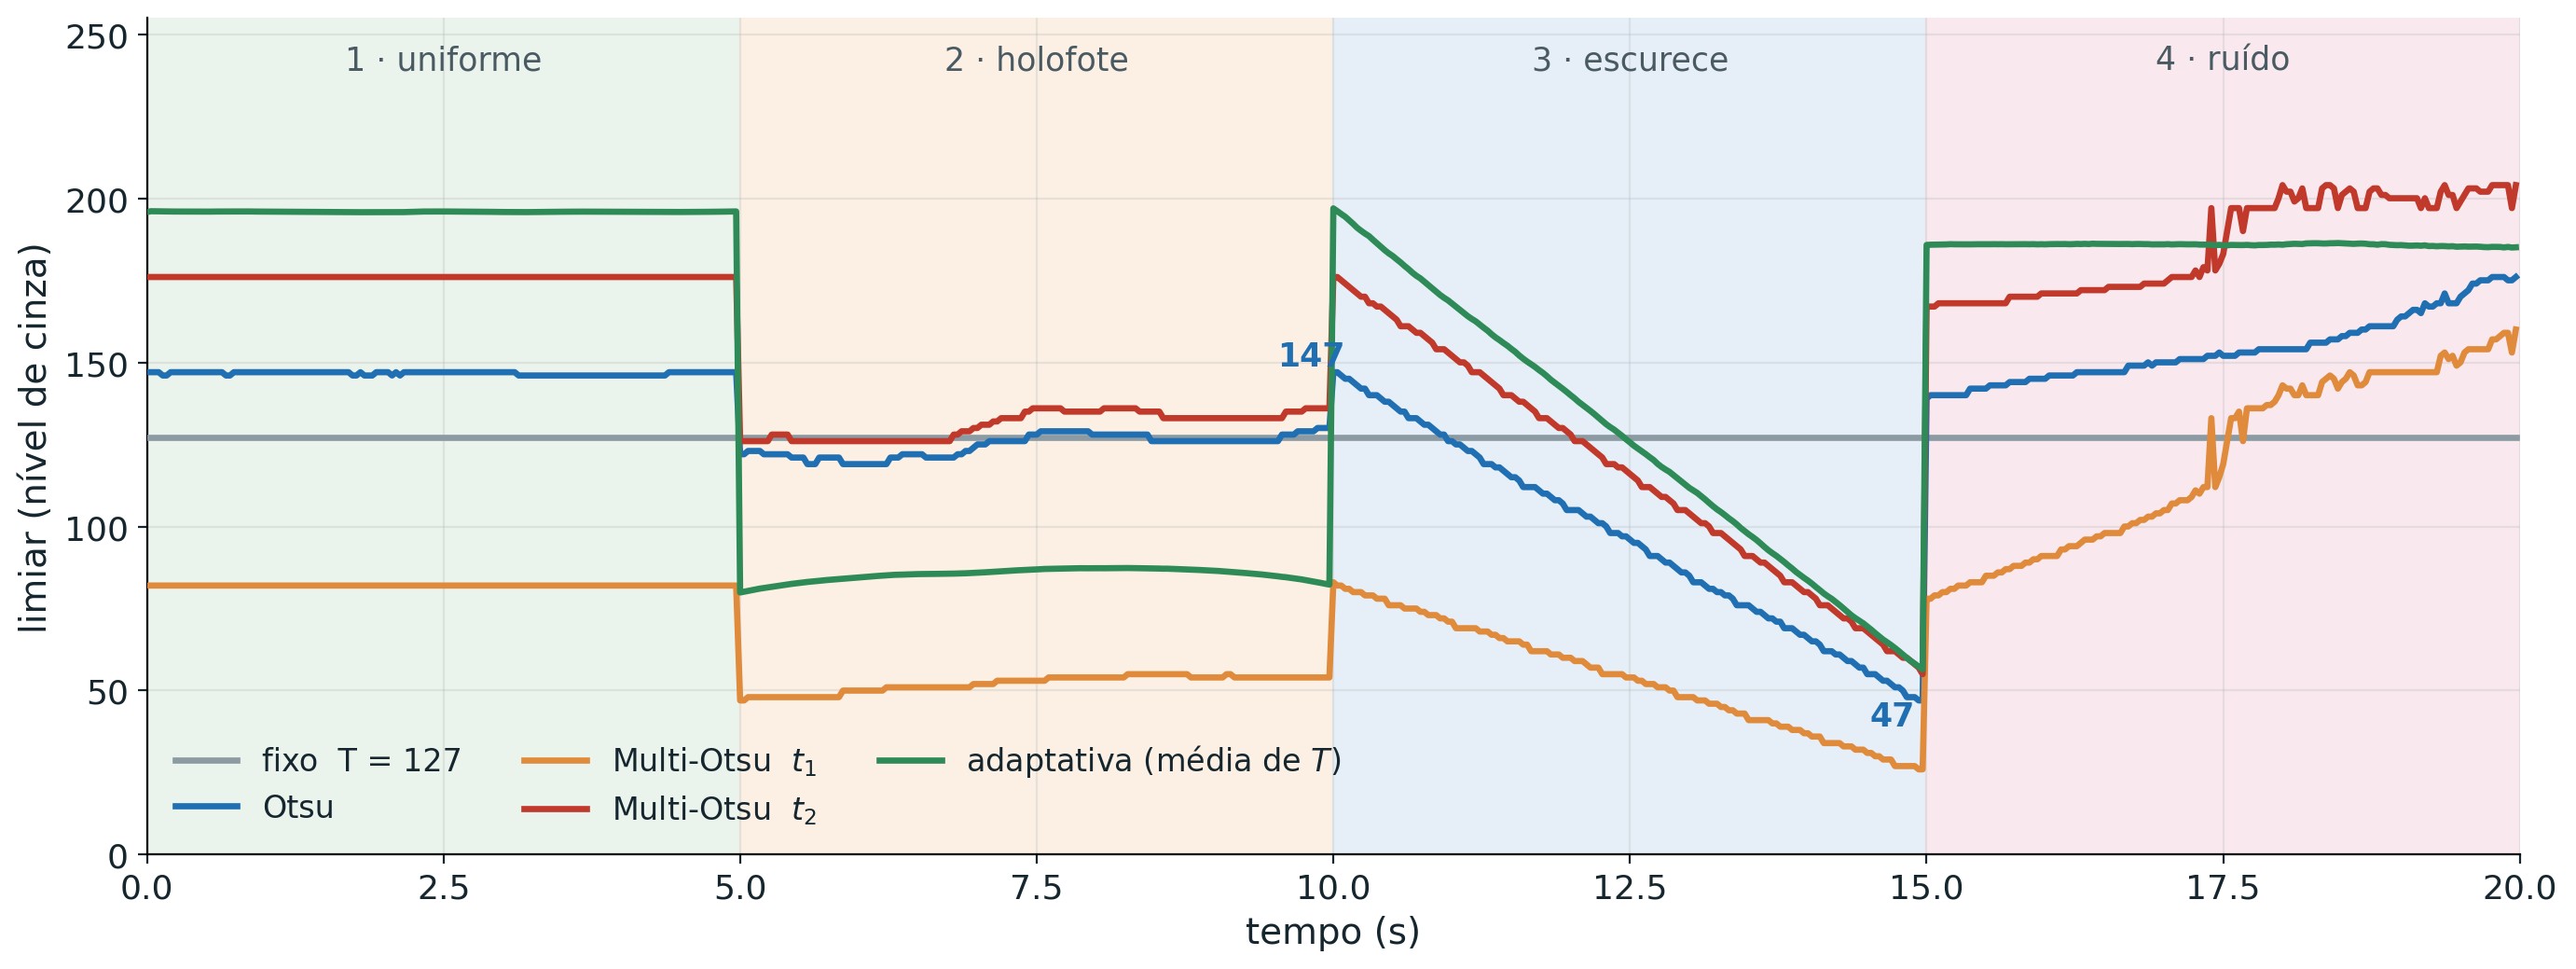
\includegraphics[width=.95\textwidth]{limiar_no_tempo_slide}
  \end{center}

  \vspace{-.4em}
  \leg{Na fase 3 a cena escurece e os métodos automáticos acompanham: o limiar
  do Otsu desce de 147 para 47 sem perda de qualidade. O limiar fixo, em cinza,
  não se move.}

\end{frame}

% -----------------------------------------------------------------------------
\begin{frame}{Resultados no vídeo}

  \begin{center}
  \small
  \begin{tabular}{@{}lccccc@{}}
    \toprule
    Método & \textbf{1} uniforme & \textbf{2} holofote & \textbf{3} escurece
           & \textbf{4} ruído & Global \\
    \midrule
    Limiar fixo $T=127$      & 0,657 & 0,140 & 0,636 & 0,634 & 0,516 \\
    Otsu                     & 0,944 & 0,139 & 0,943 & \textbf{0,834} & 0,715 \\
    Multi-Otsu $t_1$         & 0,592 & 0,731 & 0,600 & 0,639 & 0,641 \\
    Multi-Otsu $t_2$         & 0,966 & 0,138 & \textbf{0,965} & 0,626 & 0,674 \\
    Adaptativa $b{=}151$     & \textbf{0,971} & \textbf{0,956} & 0,950 & 0,575 & \textbf{0,863} \\
    \bottomrule
  \end{tabular}
  \end{center}

  \vspace{1em}
  \begin{columns}[T,onlytextwidth]
    \column{.47\textwidth}
      Na fase 2 os métodos globais colapsam e a adaptativa mantém 0,956. A
      escolha ótima de um limiar global não ajuda quando nenhum limiar único
      serve.
    \column{.47\textwidth}
      Na fase 4 a ordem se inverte. O limiar global é estimado com 307\,200
      pixels e o ruído se cancela; o local usa $b^2$ pixels e herda o ruído.
  \end{columns}

\end{frame}

% -----------------------------------------------------------------------------
\begin{frame}{Onde cada método erra}

  \vspace{-.3em}
  \begin{center}
    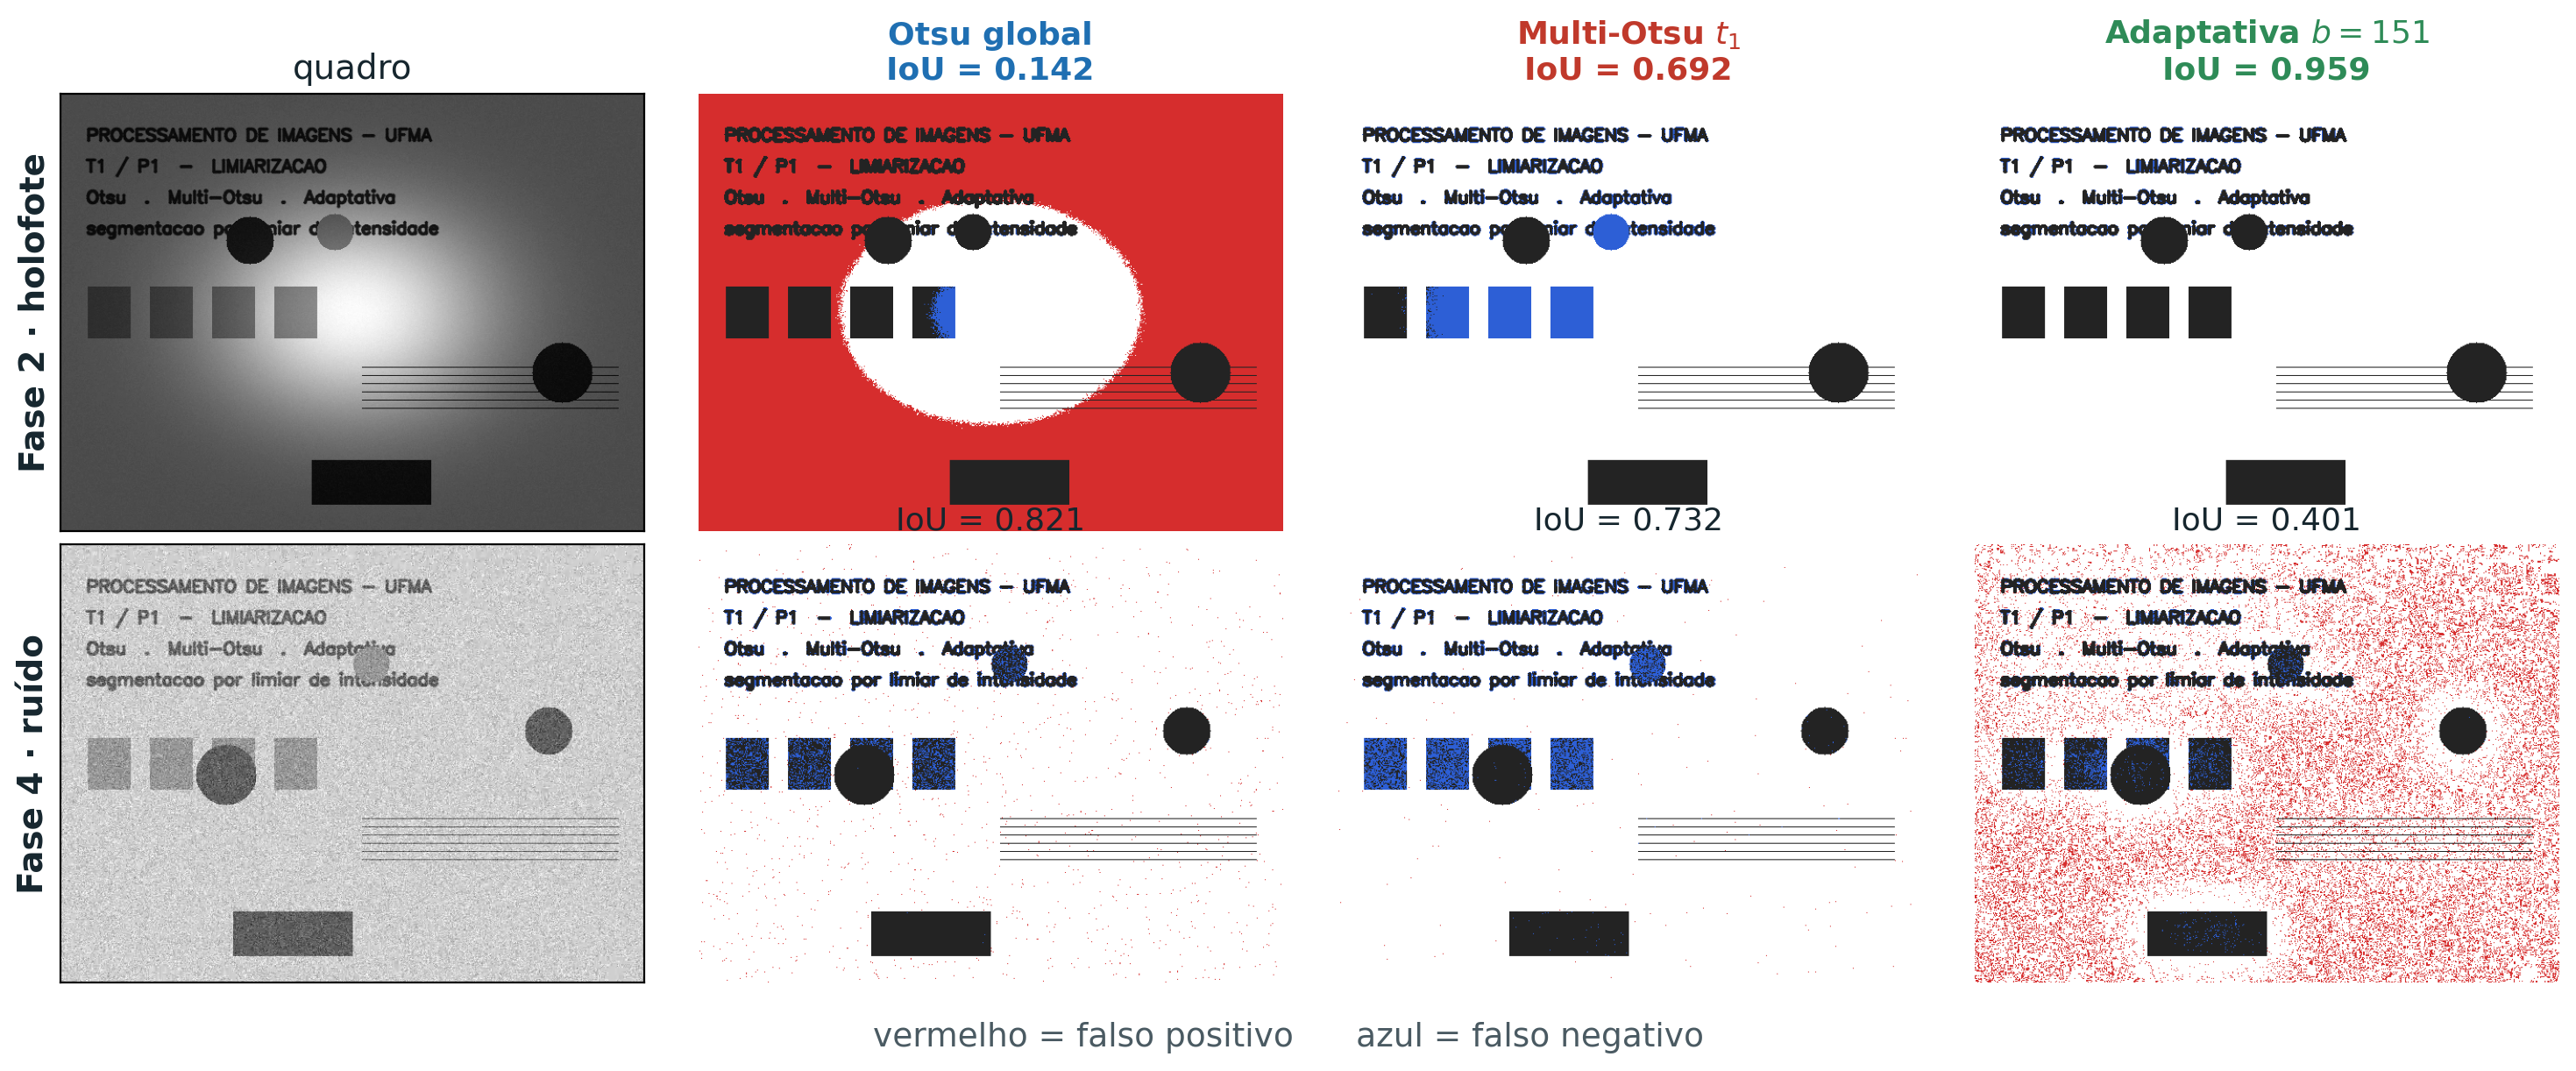
\includegraphics[width=.90\textwidth]{erros_slide}
  \end{center}

  \vspace{-.5em}
  \leg{Sob o holofote o Otsu classifica como objeto todo o fundo escurecido.
  Na fase de ruído é a adaptativa que fica coberta de falsos positivos. A ordem
  dos métodos se inverte entre as duas linhas.}

\end{frame}

% =============================================================================
\begin{frame}{Conclusão}

  \begin{itemize}
    \item O limiar global falha com variação \textbf{espacial} de iluminação,
      não com variação temporal. O mesmo Otsu obteve 0,943 na fase 3 e 0,139 na
      fase 2.

    \item A limiarização adaptativa troca robustez à iluminação por fragilidade
      ao ruído. As duas coisas vêm da mesma causa: ela decide a partir de poucos
      pixels.

    \item Nenhum método venceu as quatro fases. A escolha depende de qual
      hipótese a cena satisfaz, não de qual técnica é melhor.
  \end{itemize}

  \vspace{.8em}
  \leg{Limitações: o vídeo é sintético, escolha feita para ter gabarito exato;
  usamos um único ajuste de parâmetros por método; e não houve
  pós-processamento morfológico, que mudaria o resultado da fase 4.}

\end{frame}

% -----------------------------------------------------------------------------
\begin{frame}[standout]
  Obrigado
\end{frame}

% -----------------------------------------------------------------------------
\begin{frame}{Referências}

  \footnotesize
  \begin{itemize}
    \item Otsu, N. \emph{A Threshold Selection Method from Gray-Level
      Histograms}. IEEE Trans. SMC, 9(1):62--66, 1979.
    \item Liao, P.-S., Chen, T.-S., Chung, P.-C. \emph{A Fast Algorithm for
      Multilevel Thresholding}. J. Inf. Sci. Eng., 17:713--727, 2001.
    \item Sauvola, J., Pietikäinen, M. \emph{Adaptive Document Image
      Binarization}. Pattern Recognition, 33(2):225--236, 2000.
    \item Bradley, D., Roth, G. \emph{Adaptive Thresholding using the Integral
      Image}. J. Graphics Tools, 12(2):13--21, 2007.
    \item Gonzalez, R. C., Woods, R. E. \emph{Digital Image Processing}, cap. 10.
    \item scikit-image, \texttt{plot\_thresholding} e \texttt{plot\_multiotsu};
      OpenCV, \texttt{py\_thresholding}.
  \end{itemize}

\end{frame}

\end{document}
